\documentclass{article}

% Language setting
% Replace `english' with e.g. `spanish' to change the document language
\usepackage[english]{babel}

% Set page size and margins
% Replace `letterpaper' with `a4paper' for UK/EU standard size
\usepackage[letterpaper,top=2cm,bottom=2cm,left=3cm,right=3cm,marginparwidth=1.75cm]{geometry}

% Useful packages
\usepackage{amsmath}
\usepackage{graphicx}
\usepackage[colorlinks=true, allcolors=blue]{hyperref}

% quotes
\usepackage{dirtytalk}

% code blocks
\usepackage[outputdir=build, cachedir=build/_minted-notes]{minted}

\title{Lectures Notes on Embedded Systems}
\author{Camilo de Lellis}

\begin{document}
\maketitle

\tableofcontents

\section{Lecture - 11/09/2025}
Content taught:  Apresentação da ementa. Introdução aos sistemas embarcados, microcontroladores, conceitos e fundamentos.

\subsection{Ementa da Disciplina}
\textbf{Curso:} Curso Superior de Tecnologia em Sistemas para Internet
\textbf{Disciplina:} Sistemas Embarcados \textbf{Carga-Horária:} 60h (80h/a)
\textbf{Pré-Requisito(s):} Sistemas Digitais \textbf{Número de créditos:} 4

\begin{center}
EMENTA
\end{center}
Aspectos relacionados ao desenvolvimento de sistemas embarcados.

\begin{center}
PROGRAMA
\end{center}

\begin{center}
Objetivos
\end{center}
Conhecer técnicas e ferramentas para desenvolvimento de Sistemas Embarcados.

\begin{center}
Bases Científico-Tecnológicas (Conteúdos)
\end{center}

\begin{itemize}
      \item 1. Introdução
      \begin{itemize}
           \item 1.1. Histórico e evolução;
           \item 1.2. Características;
           \item 1.3. Aplicações típicas;
           \item 1.4. Tecnologias e Arquiteturas;
           \item 1.5. Projeto e Modelagem de Sistemas Embarcados.
      \end{itemize}
      \item 2. Hardware
      \begin{itemize}
            \item 2.1. Introdução aos microprocessadores e microcontroladores;
            \item 2.2. Dispositivos de Entrada e Saída;
            \item 2.3. Sensores;
            \item 2.4. Atuadores;
            \item 2.5. Interfaces de Comunicação.
      \end{itemize}
      \item 3. Programação
      \begin{itemize}
            \item 3.1. Ambientes de Desenvolvimento;
            \item 3.2. Principais SOs para Sistemas Embarcados;
            \item 3.3. Desenvolvimento de Sistemas Embarcados;
            \item 3.4. Conectividades;
            \item 3.5. Programação concorrente: Conceitos de concorrência, problema de exclusão mútua, comunicação e sincronização em memória compartilhada e por troca de mensagens;
            \item 3.6. Escalonamento em projetos de sistemas embarcados;
            \item 3.7. Segurança.
      \end{itemize}
\end{itemize}

\begin{center}
Procedimentos Metodológicos
\end{center}
Aulas expositivas; aulas práticas, estudos dirigidos; seminários; vídeos; dinâmicas de grupo; visitas
técnicas; palestras.

\begin{center}
Recursos Didáticos
\end{center}
Quadro branco e pincel; computador; internet; projetor de multimídia.

\begin{center}
Avaliação
\end{center}
Trabalhos práticos; apresentação de seminários; relatórios; avaliação escrita e prática.

\begin{center}
Bibliografia Básica
\end{center}
\begin{itemize}
      \item 1. ALMEIDA, Rodrigo de; MORAES, Carlos; SERAPHIM, Thatyana. Programação de Sistemas Embarcados. Editora Elsevier. 2016.
      \item 2. DENARDIN, Gustavo Weber; BARRIQUELLO, Carlos Henrique. Sistemas Operacionais de Tempo Real e sua Aplicação em Sistemas Embarcados. Editora Blucher. 2019.
      \item 3. JUNIOR, Sérgio Luiz Stevan; SILVA, Rodrigo Adamshuk. Automação e Instrumentação Industrial com Arduino: Teoria e Projetos. Editora Érica. 2015.
\end{itemize}

\begin{center}
Bibliografia Complementar
\end{center}
\begin{itemize}
      \item 1. YIU, Joseph. The Definitive Guide to ARM® Cortex®-M3 and Cortex®-M4 Processors. 3. ed. Newnes. 2013.
      \item 2. TOULSON, Rob; WILMSHURST, Tim. Fast and Effective Embedded Systems Design: Applying the ARM mbed. Editora Newnes. 2016.
      \item 3. JUCA, Sandro; PEREIRA, Renata. Aplicações Práticas de sistemas embarcados Linux utilizando Raspberry Pi. Editora PoD. 2018.
      \item 4. GU, Changyi. Building Embedded Systems: Programmable Hardware.Editora: Apress. 2016.
      \item 5. BERGER, Arnold S. Embedded Systems Design: An Introduction to Processes, Tools, and Techniques. Editora CMP Books. 2017.
\end{itemize}

\begin{center}
Software(s) de Apoio:
\end{center}
\begin{itemize}
      \item Linguagem de Programação;
      \item IDE - Ambiente de Desenvolvimento Integrado.
\end{itemize}

\subsection{Introdução aos sistemas embarcados}
Um sistema embarcado é:

\say{A combination of computer hardware and software, and perhaps additional mechanical or other parts, designed to perform a dedicated function. In some cases, embedded systems are part of a larger system or product, as in the case of an antilock braking system in a car.}
-- Michael Barr

Exemplos de sistemas embarcados são:

\say{ Microwave ovens, cell phones, calculators, digital watches, VCRs, cruise missiles, GPS receivers, heart monitors, laser printers, radar guns, engine controllers, digital cameras, traffic lights, remote controls, bread machines, fax machines, pagers, cash registers, treadmills, gas pumps, credit/debit card readers, thermostats, pacemakers, blood gas monitors, grain analyzers, and a gazillion others.}
-- Michael Barr

\subsection{Introdução a microcontroladores}
Um microcontrolador é:

\say{A highly integrated microprocessor designed specifically for use in embedded systems. Microcontrollers typically include an integrated CPU, memory (a small amount of RAM, ROM, or both), and other peripherals on the same chip. Common examples are Microchip's PIC, the 8051, Intel's 80196, and Motorola's 68HCxx series.}
-- Michael Barr

\begin{figure}
\centering
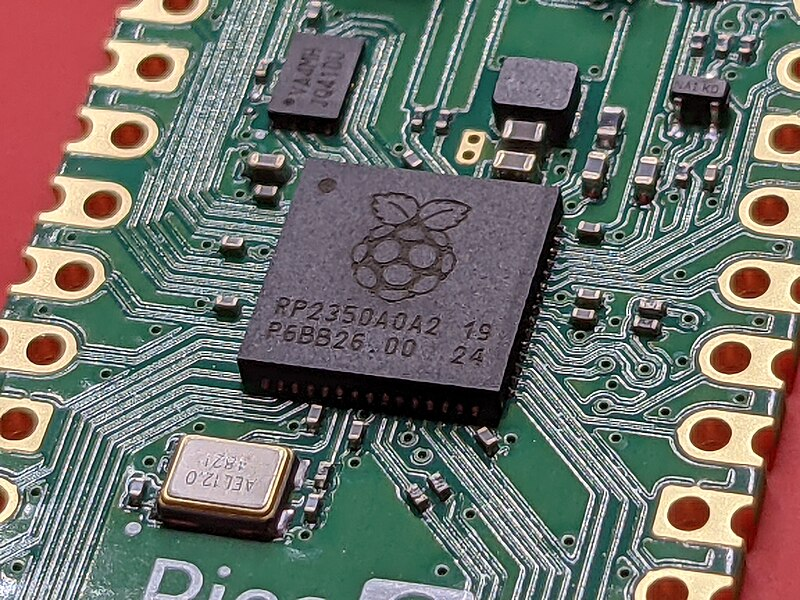
\includegraphics[width=0.25\linewidth]{./images/pi_pico_mc.jpg}
\caption{\label{fig:rp2305}This is the RP2350 microcontroller chip seen in the circuit board of a Raspberry Pi Pico 2.}
\end{figure}

\subsection{Conceitos e fundamentos}
...

\section{Lecture - 15/09/2025}
Content taught:  Conceitos básicos sobre sistemas embarcados - entradas digitais. 

\subsection{Entradas Digitais}
...

\section{Lecture - 18/09/2025}
Content taught:  Introdução à programação de microcontroladores em linguagem C: tipos de dados; tabela ASCII e sistema binário; configuração de GPIO.

\subsection{Introdução à programação de microcontroladores em linguagem C}
...

\subsubsection{Tipos de dados} 
...

\subsubsection{Tabela ASCII e Sistema Binário}
...

\subsubsection{Configuração de GPIO}
...

\section{Lecture - 22/09/2025}
Content taught:  Manipulando saídas digitais: Acionamento de LED; corrente máxima nos pinos; cálculo da resistência limitadora. Prática rápida: Implementação de um circuito de sinalização de entrada e saída de veículos. Interface entre circuitos digitais e cargas de alta potência utilizando transistores: Transistor como chave eletrônica; Acionamento de motores CC. 

\subsection{Manipulando saídas digitais}
...

\subsubsection{Acionamento de LED}
...

\subsubsection{Corrente máxima nos pinos}
...

\subsubsection{Cálculo da resistência limitadora}
...

\subsubsection{Prática rápida}
...

\paragraph{Implementação de um circuito de sinalização de entrada e saída de veículos}
...

\paragraph{Interface entre circuitos digitais e cargas de alta potência utilizando transistores}
...

\paragraph{Transistor como chave eletrônica}
...

\paragraph{Acionamento de motores CC}
...

\section{Lecture - 25/09/2025}
Content taught:  Programação de microcontroladores: temporização. Funções delay() e millis(). Espera ocupada.

\subsection{Programação de microcontroladores: Temporização}
...

\subsubsection{Função delay()}
...

\subsubsection{Função millis()}
...

\subsubsection{Espera ocupada}
...


\section{Lecture - 29/09/2025}
Content taught: Prática sobre acinamento de cargas utilizando transistores. Os alunos tiveram um primeiro contato com o laboratório de eletrônica, onde montaram um circuito simples de ativação de uma ventoinha por meio do chaveamento de um transistor de potência. O intuito da aula foi preparar a turma para futuras práticas de acionamento utilizando programação e transistores. Trabalhou-se a competência de se interpretar um esquema eletrônico, bem como de criar novos arranjos de acordo com uma necessidade específica.

\subsection{Prática sobre acinamento de cargas utilizando transistores}
...

\section{Lecture - 02/10/2025}
Content taught: Programação com temporização: função millis().

\subsection{Programação com temporização: função millis()}
...

\section{Lecture - 06/10/2025}
Content taught: Exercícios sobre entradas digitais, saídas, resistores de pull-lup, pull-down, projeto de sistemas digitais utilizando arduino; Utilização dos operadores lógicos da linguagem C.

\subsection{Exercícios}
...

\subsubsection{Entradas digitais}
...

\subsubsection{Saídas digitais}
...

\subsubsection{Resistores de pull-up}
...

\subsubsection{Resistores de pull-down}
...

\subsubsection{Projeto de sistemas digitais utilizando arduino}
...

\subsubsection{Utilização dos operadores lógicos da linguagem C}
...


\section{Lecture - 09/10/2025}
Content taught: Programação com temporização: função millis(). Aplicações.

\subsection{Programação com temporização: função millis(). Aplicações}
...

\section{Lecture - 13/10/2025}
Content taught: Acionamento de cargas utilizando relé: Princípio de funcionamento dos relés eletromecânicos; simbologia; exemplo de aplicação.

\subsection{Acionamento de cargas utilizando relé eletromecânicos}
...

\subsubsection{Princípio de funcionamento}
...

\subsubsection{Simbologia}
...

\subsubsection{Exemplo de aplicação}
...


\section{Assignment - 17/10/2025}
Assignment Description: Considerando o contexto da aula do dia 13/10, que tratou sobre os relés, faça o que se pede nos itens abaixo:

\textbf{1. Implemente um código simples que inverte o estado da lâmpada caso um botão seja
pressionado.}
\begin{itemize}
      \item Seguir esquema mostrado em aula;
      \item Materiais utilizados: Arduino Uno, pushbutton, relé SPDT, resistor, diodo, lâmpada incandescente, transistor NPN e bateria de 9V.
\end{itemize}

\textbf{2. Envie o link da simulação.}

\subsection{Código em C++}
\begin{minted}{c}
// atribuição dos pinos
const int btn_pin = 2;
const int tst_pin = 3;

// atribuindo timestamp inicial
unsigned long millisNow = millis();
unsigned long lastMillis = millis();

// função para ler botão
void readButton(int time){
  millisNow = millis();
  if (millisNow - lastMillis >= time){
  	digitalWrite(tst_pin, !digitalRead(tst_pin));
    lastMillis = millisNow;
  }
}

// configuração incial
void setup()
{
  pinMode(btn_pin, INPUT);
  pinMode(tst_pin, OUTPUT);
  digitalWrite(btn_pin, LOW);
  digitalWrite(tst_pin, LOW);
}

// loop principal
void loop()
{
  if (digitalRead(btn_pin)){
    readButton(200); // duplo clique no intervalo de 200ms é considerado como um único clique
  }
}
\end{minted}

\section{Simulado da 1ª avaliação - 20/10/2025}
...

\section{Assignment - 23/10/2025}
This assignment was aimed to reverse engineer the game called \href{https://en.wikipedia.org/wiki/Simon_(game)}{Genius} from the traditional toy brazilian manufacturer \href{https://en.wikipedia.org/wiki/Estrela_(company)}{Estrela}. Actually, as I take these notes, just found that this game was actually international.

Simon is a short term memory electronic game \cite{wikipedia_simon}. It was patent under  Ralph H. Baer and Howard J. Morrison \cite{simon_patent}. The game loop is pretty simple, according to Wikipedia: \\"The device creates a series of tones and lights and requires a user to repeat the sequence. If the user succeeds, the series becomes progressively longer and more complex. Once the user fails or the time limit runs out, the game is over." \cite{wikipedia_simon}

The full simulation for our recreation is available publicy at \href{https://www.tinkercad.com/things/5QbNWprTGky-genius-estrela?sharecode=emlPcyX6GBUJY967Q9LnX9mBZDVs0M2osP7Pup8dmDg}{Tinkercad}. Also, the \href{https://github.com/delellisc/embedded-systems/blob/master/genius-estrela/genius-estrela.ino}{full code}  written is available at this remote repository too.

\begin{figure}
\centering
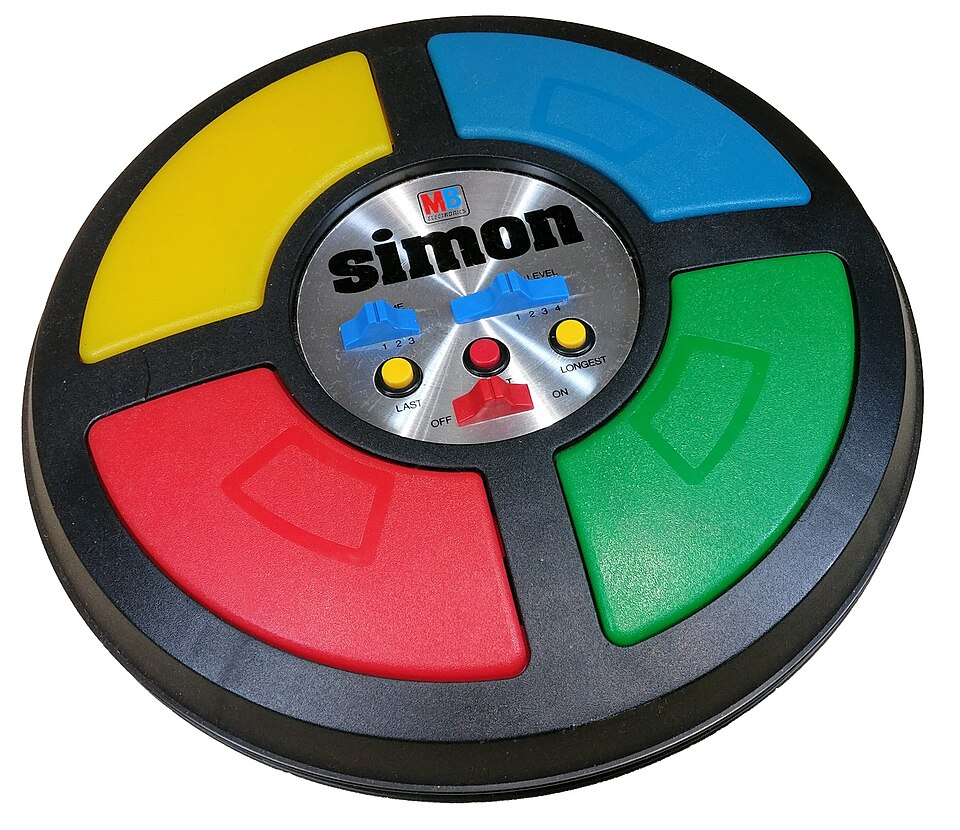
\includegraphics[width=0.25\linewidth]{./images/simon_electronic_game.jpg}
\caption{\label{fig:simon-game}This is the Simon electronic game, also called Genius in Brazil.}
\end{figure}

\section{Lecture - 30/10/2025}
Content taught: Presentation of the updated version of last assignment. Introduction to Analog Inputs.

Updated code:
\begin{minted}{cpp}
int read_btn(int btn_pin){
    millisATUAL = millis();
        while(millisATUAL - millisANT <= 10000){
            millisATUAL = millis();
            if (digitalRead(btn_pin)){
                Serial.print("ACERTO");
                // returns 1 only when right
                return 1;
            }
            else if(
                btn_pin != btn_red && digitalRead(btn_red) ||
                btn_pin != btn_grn && digitalRead(btn_grn) ||
                btn_pin != btn_yel && digitalRead(btn_yel) ||
                btn_pin != btn_ble && digitalRead(btn_ble)
            ){
                Serial.print("ERRO\n");
                return 0;
            }
        }
    // returns 0 if no condition is met    
    return 0;
}
\end{minted}

\href{https://en.wikipedia.org/wiki/IEEE_754}{Floating point number arithmetic}...

To represent floating point numbers, we need the least significant bit to be less than 2 to the power of 0.

Arduino UNO has a resolution of 10 bits. 

\section{\LaTeX}
I shall take notes with \LaTeX and then convert them to Markdown. To convert it into my README.md, I’ll just use the following:

\begin{minted}{bash}
pandoc main.tex -o README.md --from=latex --to=gfm
\end{minted}

\bibliographystyle{plain}
\bibliography{references}

\end{document}
